\documentclass{beamer}
\usetheme{metropolis}  % https://github.com/matze/mtheme
\usepackage{hyperref}
\usepackage[utf8]{inputenc} % this is needed for german umlauts
\usepackage[english]{babel} % this is needed for german umlauts
\usepackage[T1]{fontenc}    % this is needed for correct output of umlauts in pdf

\usepackage{adjustbox}
\usepackage{tikz}
\usetikzlibrary{mindmap,trees}

\begin{document}

\title{Data Science}
\subtitle{Tasks, Tools and Roles}
\author{Martin Thoma}
\date{3. September 2019}
\subject{Computer Science; Business}

\frame{\titlepage}

\begin{frame}[plain]{}
    \begin{center}\Huge
    Hi. \uncover<2->{I'm Martin.}
    \end{center}
\end{frame}

\begin{frame}[plain]{}
    \begin{center}\huge
    \uncover<1->{I'm a Data Scientist.\\}
    \uncover<2->{Or Machine Learning Engineer?\\}
    \uncover<3->{Or Business Analyst?\\}
    \uncover<4->{Or Data Engineer?}
    \end{center}
\end{frame}


\begin{frame}[plain]{}
    \begin{adjustbox}{max totalsize={.99\textwidth}{.99\textheight},center}
    
\begin{tikzpicture}
      \path[mindmap,concept color=black,text=white]
        node[concept] {Data Science};
    \end{tikzpicture}
    \end{adjustbox}
\end{frame}

\begin{frame}[plain]{}
    \begin{adjustbox}{max totalsize={.99\textwidth}{.99\textheight},center}
    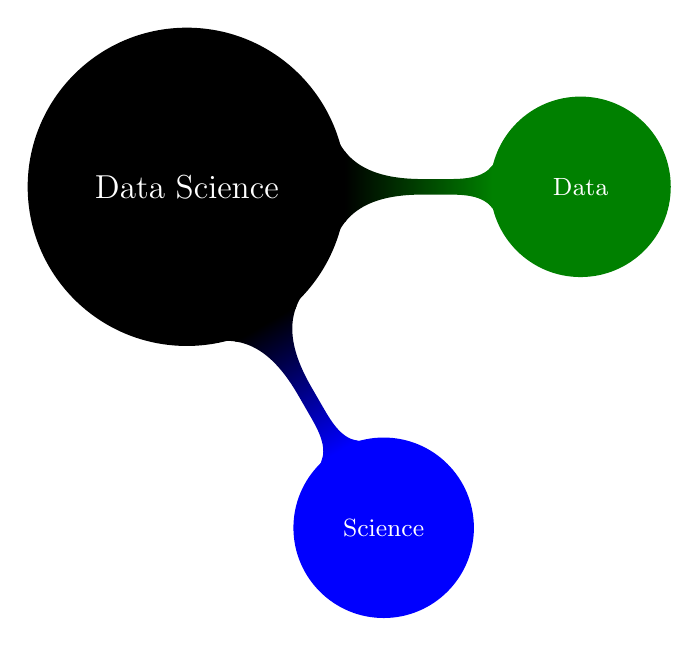
\begin{tikzpicture}
      \path[mindmap,concept color=black,text=white]
        node[concept] {Data Science}
        [clockwise from=0]
        child[concept color=green!50!black] {
          node[concept] {Data}
        }
        child[concept color=blue] {
          node[concept] {Science}
        };
    \end{tikzpicture}
    \end{adjustbox}
\end{frame}

\begin{frame}[plain]{}
    \begin{adjustbox}{max totalsize={.99\textwidth}{.99\textheight},center}
    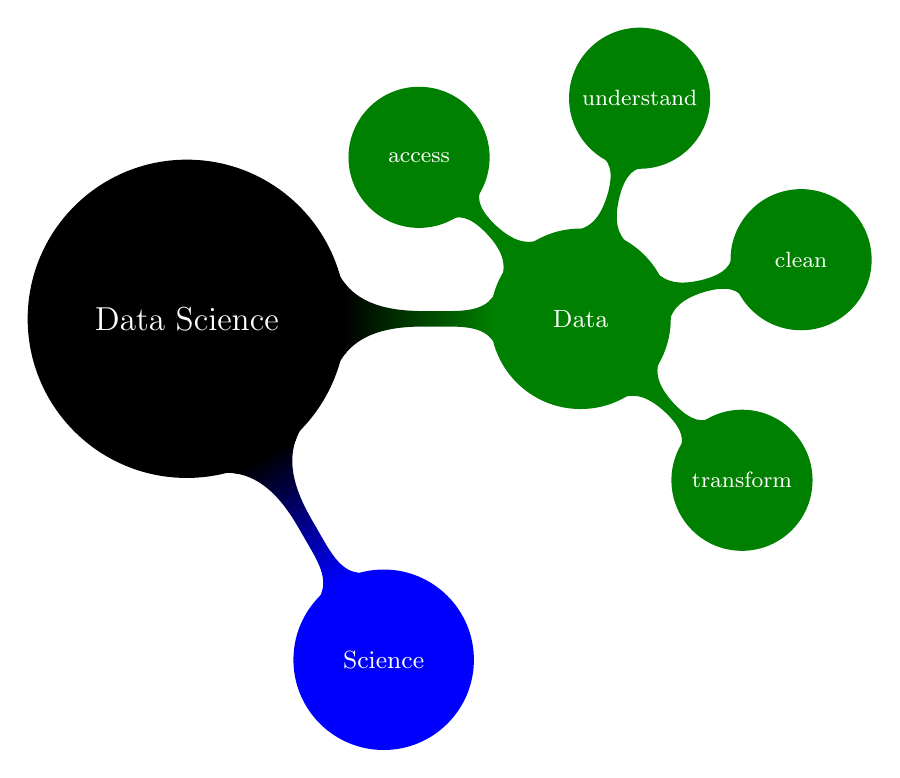
\begin{tikzpicture}
      \path[mindmap,concept color=black,text=white]
        node[concept] {Data Science}
        [clockwise from=0]
        child[concept color=green!50!black] {
          node[concept] {Data}
          [clockwise from=135]
          child { node[concept] {access} }
          child { node[concept] {understand} }
          child { node[concept] {clean} }
          child { node[concept] {transform} }
        }
        child[concept color=blue] {
           node[concept] {Science}
        };
        % child[concept color=red] { node[concept] {technical} }
        % child[concept color=orange] { node[concept] {theoretical} };
    \end{tikzpicture}
    \end{adjustbox}
\end{frame}

\begin{frame}[plain]{}
    \begin{adjustbox}{max totalsize={.99\textwidth}{.99\textheight},center}
    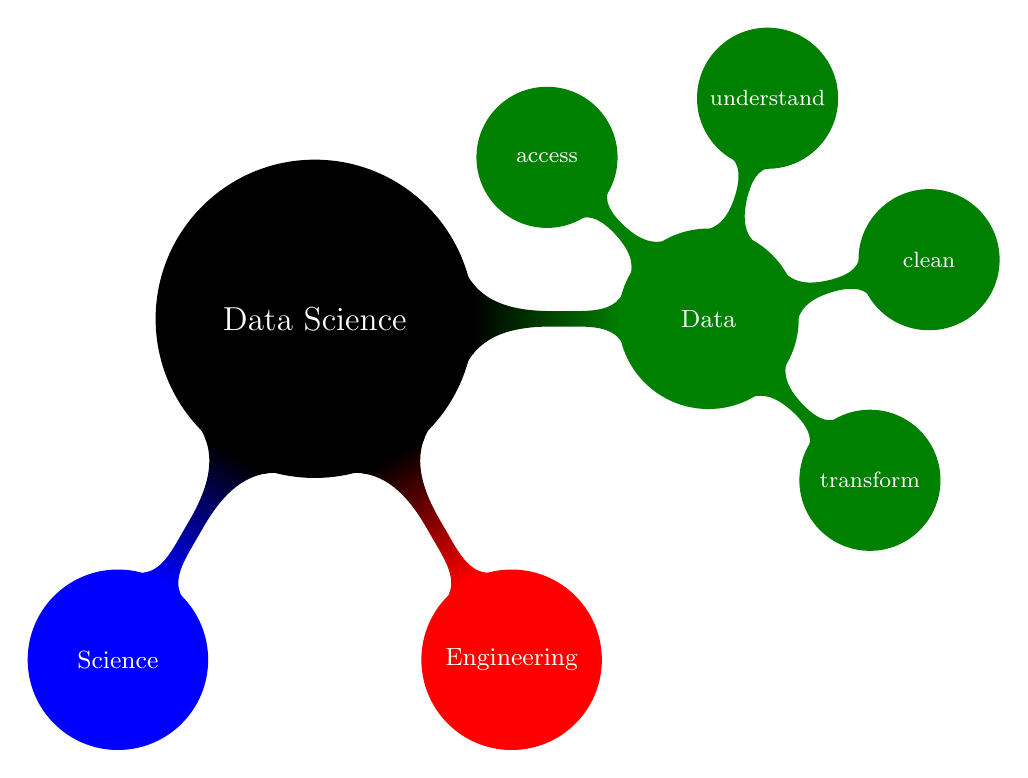
\begin{tikzpicture}
      \path[mindmap,concept color=black,text=white]
        node[concept] {Data Science}
        [clockwise from=0]
        child[concept color=green!50!black] {
          node[concept] {Data}
          [clockwise from=135]
          child { node[concept] {access} }
          child { node[concept] {understand} }
          child { node[concept] {clean} }
          child { node[concept] {transform} }
        }
        child[concept color=red] {
          node[concept] {Engineering}
        }
        child[concept color=blue] {
          node[concept] {Science}
        };
        % child[concept color=orange] { node[concept] {theoretical} };
    \end{tikzpicture}
    \end{adjustbox}
\end{frame}

\begin{frame}[plain]{}
    \begin{adjustbox}{max totalsize={.99\textwidth}{.99\textheight},center}
    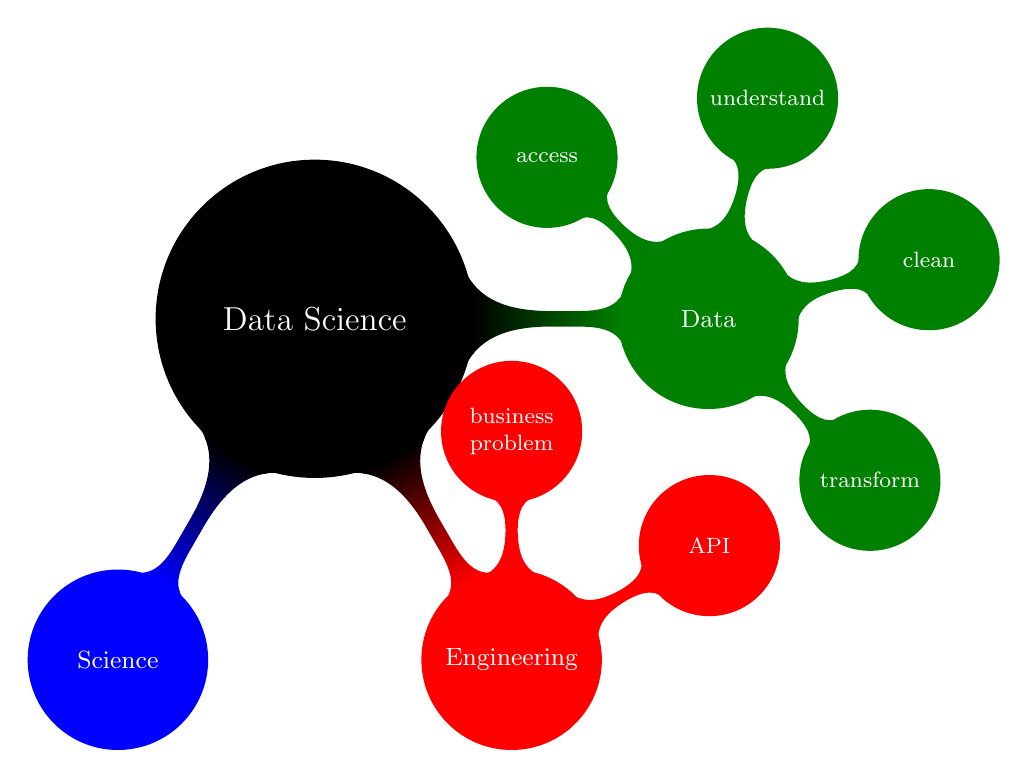
\begin{tikzpicture}
      \path[mindmap,concept color=black,text=white]
        node[concept] {Data Science}
        [clockwise from=0]
        child[concept color=green!50!black] {
          node[concept] {Data}
          [clockwise from=135]
          child { node[concept] {access} }
          child { node[concept] {understand} }
          child { node[concept] {clean} }
          child { node[concept] {transform} }
        }
        child[concept color=red] {
          node[concept] {Engineering}
          [clockwise from=90]
          child { node[concept] {business problem} }
          child { node[concept] {API} }
        }
        child[concept color=blue] {
          node[concept] {Science}
        };
        % child[concept color=orange] { node[concept] {theoretical} };
    \end{tikzpicture}
    \end{adjustbox}
\end{frame}

\begin{frame}[plain]{}
    \begin{adjustbox}{max totalsize={.99\textwidth}{.99\textheight},center}
    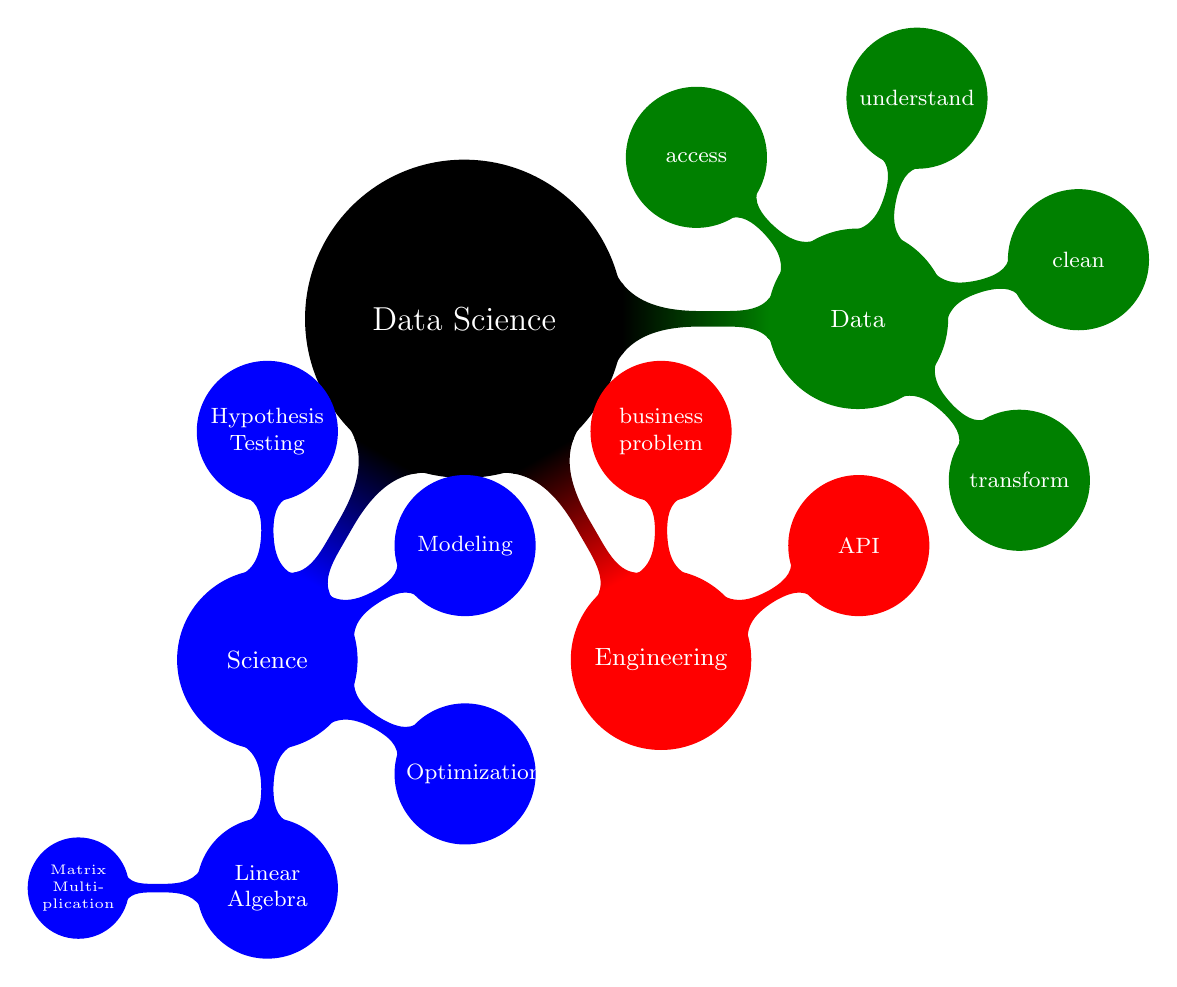
\begin{tikzpicture}
      \path[mindmap,concept color=black,text=white]
        node[concept] {Data Science}
        [clockwise from=0]
        child[concept color=green!50!black] {
          node[concept] {Data}
          [clockwise from=135]
          child { node[concept] {access} }
          child { node[concept] {understand} }
          child { node[concept] {clean} }
          child { node[concept] {transform} }
        }
        child[concept color=red] {
          node[concept] {Engineering}
          [clockwise from=90]
          child { node[concept] {business problem} }
          child { node[concept] {API} }
        }
        child[concept color=blue] {
          node[concept] {Science}
          [clockwise from=90]
          child { node[concept] {Hypothesis Testing} }
          child { node[concept] {Modeling} }
          child { node[concept] {Optimization} }
          child[concept] {
              node[concept] {Linear Algebra}
              [clockwise from=180]
              child { node[concept] {Matrix Multiplication} }
              }
        };
        % child[concept color=orange] { node[concept] {theoretical} };
    \end{tikzpicture}
    \end{adjustbox}
\end{frame}

\begin{frame}[plain]{}
    \begin{tabular}{l|ll}
                & \textbf{Data Engineer} & \textbf{Data Scientist} \\
    Buzz Words  & Big Data, Data Lake    & AI, DL, Neural Networks \\
    Background  & Computer Science       & Computer Science        \\
    Languages   & Java, Python           & Python, R               \\
    Tools       & Spark, Hadoop          & Tensorflow, Keras, Sklearn \\
    Solutions   & Data Accessible        & Predictive Model        \\
    \end{tabular}
\end{frame}

\begin{frame}[plain]{}
    \begin{tabular}{l|ll}
                & \textbf{Data Analyst}     & \textbf{Data Scientist} \\
                & \textbf{Business Analyst} &       \\
    Buzz Words  & Data Warehouse            & AI, Deep Learning, NNs \\
    Background  & Mathematics, economics    & Computer Science \\
    Languages   & Excel, Python, R          & Python, R           \\
    Tools       & Tableau, QlikView         & Pandas, Jupyter, Sklearn \\
    Solutions   & Business Decision         & Predictive Model        \\
    \end{tabular}
\end{frame}

\begin{frame}[plain]{}
    \begin{center}
        \huge ML Engineer
        \normalsize
        \begin{itemize}
            \item Refactor / Productionalize Data Scientists Code
            \item Glorified Software Engineer who stumbled into Data Science
        \end{itemize}
        \tiny
        Sources: 

        \begin{itemize}
            \item /r/MachineLearning: \href{https://www.reddit.com/r/MachineLearning/comments/cxhvbd/}{What is the reality of machine learning engineer?}
            \item Tomasz Dudek: \href{https://medium.com/@tomaszdudek/but-what-is-this-machine-learning-engineer-actually-doing-18464d5c699}{But what is this “machine learning engineer” actually doing?}
        \end{itemize}
    \end{center}
\end{frame}

\begin{frame}{Use Cases}
    \begin{itemize}
        \item \textbf{Time Series}: How many calls will our call center get?
        \item \textbf{Categorization}: What topic is an e-mail / tweet / a comment about?
        \item \textbf{Recommendations}: What do I want to buy? What should I watch next?
        \item \textbf{Information Retrival}: (Fuzzy) Search, Lookup, Autocomplete
    \end{itemize}
\end{frame}

\begin{frame}{Hard Use Cases}
    \begin{itemize}
        \item \textbf{Automatic Speech Recognition}: Speech to Text
        \item \textbf{Speech Synthesis}: Text to Speech
        \item \textbf{Translation}
    \end{itemize}
\end{frame}

\begin{frame}{Typical Problems}
    \begin{itemize}
        \item Data Access / Availability
        \item Data Understanding
        \item Dirty Data
        \item Problem Definition / Optimization Metric
        \item When is it good enough?
    \end{itemize}
\end{frame}

%%%%%%%%%%%%%%%%%%%%%%%%%%%%%%%%%%%%%%%%%%%%%%%%%%%%%%%%%%%%%%%%%%%%%%%%%%%%%%%
\end{document}
